\documentclass[12pt]{article}
\usepackage[utf8]{inputenc}

\usepackage{float}
\usepackage{amsmath}
\usepackage{fullpage}
\usepackage{amsfonts, amsmath, pifont}
\usepackage{amsthm}
\usepackage{graphicx}
\usepackage{float}

\usepackage{tkz-euclide}
\usepackage{tikz}
\usepackage{pgfplots}
\pgfplotsset{compat=1.13}


\usepackage[hmargin=3cm,vmargin=6.0cm]{geometry}
%\topmargin=0cm
\topmargin=-2cm
\addtolength{\textheight}{6.5cm}
\addtolength{\textwidth}{2.0cm}
%\setlength{\leftmargin}{-5cm}
\setlength{\oddsidemargin}{0.0cm}
\setlength{\evensidemargin}{0.0cm}

%misc libraries goes here




\begin{document}

\section*{Student Information } 
%Write your full name and id number between the colon and newline
%Put one empty space character after colon and before newline
%Full Name : Ömer Kılınç \\
%Id Number : 2448603 \\

% Write your answers below the section tags
\section*{Answer 1} 


\[
x(t) = 
\begin{array}{cc}
  \{ & 
    \begin{array}{cc}
      1 & -3 \leq t \leq 7 \\
      0 & otherwise
    \end{array}
\end{array}
\]

\[
h(t) =
\begin{array}{cc}
  \{ & 
    \begin{array}{cc}
      1 & 1 \leq t \leq 15 \\
      0 & otherwise
    \end{array}
\end{array}
\]

\[ \textbf{Three ranges of t values, integrated seperately:}\]

\[-3\leq \tau \leq 7\]
\[t-15\leq \tau \leq t-1\]

\[ \textbf{(I)   partially overlap: } -2\leq t \leq 8 \]
\[-3\leq \tau \leq t-1\]
\[\int_{-3}^{t-1}{d\tau} = t+2\]

\[ \textbf{(II)  fully overlap: } 8\leq t \leq 12 \]
\[-3\leq \tau \leq 7\]
\[\int_{-3}^{7}{d\tau} = 10\]

\[ \textbf{(III) partially overlap: } 12\leq t \leq 22 \]
\[t-15\leq \tau \leq 7\]
\[\int_{t-15}^{7}{d\tau} = 22-t\]

\begin{figure}[h!]
    \centering
        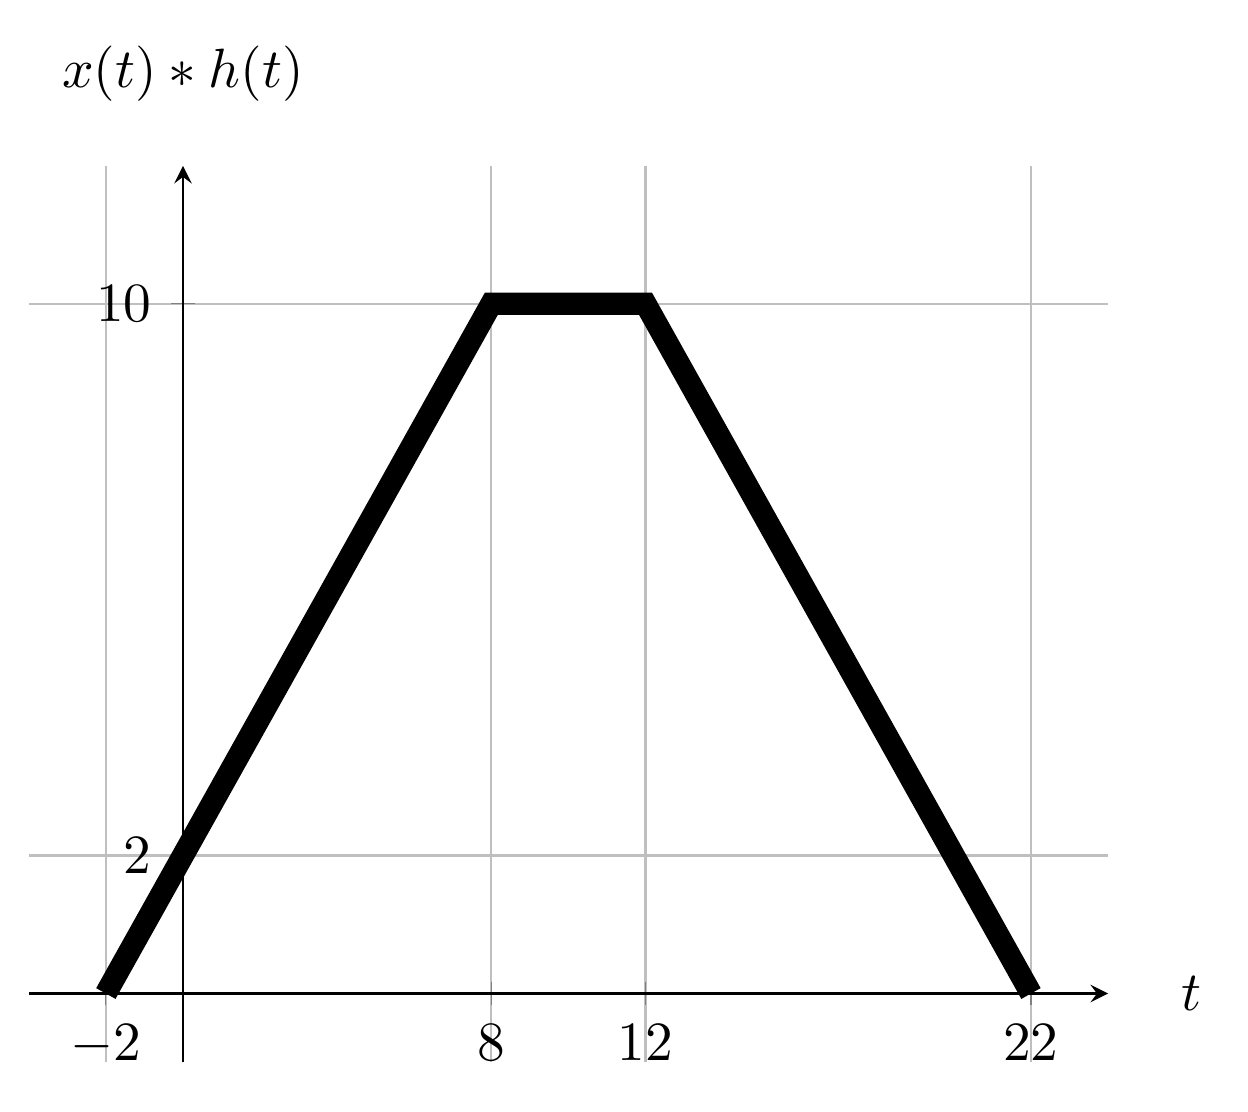
\begin{tikzpicture}[scale=2.0]
           \begin{axis}[
          axis lines=middle,
          xlabel={$t$},
          ylabel={$x(t)*h(t)$},
          xtick={-2, 8, 12, 22},
          ytick={0, 2, 10},
          ymin=-1, ymax=12,
          xmin=-4, xmax=24,
          every axis x label/.style={at={(ticklabel* cs:1.05)}, anchor=west,},
          every axis y label/.style={at={(ticklabel* cs:1.05)}, anchor=south,},
          grid,
        ]
           \path[draw,line width=4pt] (-2,0) -- (8,10) -- (12,10) -- (22,0);
           \end{axis}
        \end{tikzpicture}
        \caption{$t$ vs. $x(\frac{1}{2}t-2) $.}
        \label{fig:q2}
    \end{figure}


\end{document}


